\documentclass[crop,tikz]{standalone}

\usepackage{tikz}

\begin{document}

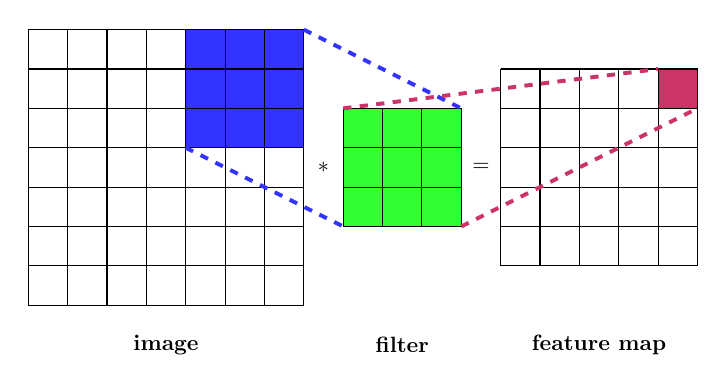
\begin{tikzpicture}[scale=0.5, every node/.style={scale=0.8}]
\draw [fill=blue!80] (0,0) grid (7,7) rectangle (4,4);
\draw [fill=green!80] (8,2) grid (11,5) rectangle (8,2);
\draw [fill=purple!80] (12,1) grid (17,6) rectangle (16,5);

\draw [-, line width=.5mm, dashed, blue!80] (7, 7) -- (11, 5);
\draw [-, line width=.5mm, dashed, blue!80] (4, 4) -- (8, 2);

\draw [-, line width=.5mm, dashed, purple!80] (8, 5) -- (16, 6);
\draw [-, line width=.5mm, dashed, purple!80] (11, 2) -- (17, 5);

\node (conv) at (7.5, 3.5) {$*$};
\node (eq) at (11.5, 3.5) {$=$};

\node (flatten) at (3.5, -1.) {\textbf{image}};
\node (flatten) at (9.5, -1.) {\textbf{filter}};
\node (flatten) at (14.5, -1.) {\textbf{feature map}};

\end{tikzpicture}

\end{document}